\documentclass[12pt]{article}
\usepackage{amsmath}
\usepackage{amssymb}
\usepackage{amsfonts}
\usepackage[polish]{babel}
\usepackage[utf8]{inputenc}
\usepackage[OT4]{fontenc}
\usepackage{graphicx}
\usepackage[cp1250]{inputenc}
\usepackage{caption}
\usepackage{float}


\captionsetup[table]{name=Tabela}


\textheight 23.2 cm

\textwidth 6.0 in

\hoffset = -0.5 in

\voffset = -2.4 cm

\hyphenation{me-to-dy la-bo-ra-to-rium}

\begin{document}

%hê?
%\thispagestyle{empty}

\vspace*{3ex}
\begin{flushright}
{\large 14 grudnia 2022 r.}
\end{flushright}

\begin{flushleft}
{\large Marta Szuwarska\\
Grupa 1 (środa 14:15)}
\end{flushleft}

\hskip3cm

\begin{center}

\Large {\bf Obliczanie całek funkcji dwóch zmiennych z zastosowaniem złożonych kwadratur prostokątów (z punktem środkowym)}

\vskip2ex

{\large Projekt nr 1}

\end{center}

\vskip20ex



\section{Opis metody}

\noindent Celem zadania jest obliczanie całek  $\iint_D \textbf{f(x,y)}d\textbf{x}d\textbf{y}$, gdzie $f : \mathbb{R}^2 \to \mathbb{R}$ jest funkcją całkowalną oraz $D = \{(x,y) \in \mathbb{R}^2 : x^2+y^2 \leq 1\}$; przez transformację na prostokąt $[0,1] \times [0,2\pi]$ (współrzędne biegunowe) i zastosowanie złożonych kwadratur prostokątów (z punktem środkowym) ze względu na każdą zmienną).
\vskip3ex
Zacznijmy od zmiany zmiennych na współrzędne biegunowe:

\vskip3ex
$\left\{ \begin{array}{ll}
x = r\cos{\varphi} \\
y = r\sin{\varphi}
\end{array} \right.$, gdzie $r \in [0,1], \varphi \in [0,2\pi]$.

\vskip3ex
Jakobian tego przekształcenia wynosi:

$J(r,\phi) = \det{\begin{vmatrix}{\frac{\partial x}{\partial r}}&{\frac{\partial x}{\partial \phi}}\\ {\frac{\partial y}{\partial r}}&{\frac{\partial y}{\partial \phi}}\end{vmatrix}} = \det{\begin{vmatrix}{\cos{\phi}}&{-r\sin{\phi}}\\ {\sin{\phi}}&{r\cos{\phi}}\end{vmatrix}} = r $
\vskip3ex
Zatem po przekształceniu całka wynosi:
\begin{equation}
    \iint_D \textbf{f(x,y)}d\textbf{x}d\textbf{y} = \int_0^1\int_0^{2\pi}rf(r\cos{\varphi},r\sin{\varphi})d\textbf{r}d\varphi = \int_0^1\int_0^{2\pi}g(r,\varphi)d\textbf{r}d\varphi
\end{equation}
\vskip3ex
gdzie $g : [0,1]\times[0,2\varphi] \to \mathbb{R}$, $g(r,\varphi) = rf(r\cos{\varphi},r\sin{\varphi})$

\vskip3ex
Dla dowolnej funkcji $f: [a,b] \to \mathbb{R}$ złożona kwadratura prostokątów (z punktem środkowym) ma postać:
\vskip3ex
$S(f) = \Sigma_{k=1}^{N}(x_k-x_{k-1})f(\frac{x_k+x_{k-1}}{2})$, 
gdzie $x_k=a+kH$ dla $k = 0,...,N$ oraz $H = \frac{b-a}{N}$.
\vskip3ex
Po przekształceniach:
\begin{equation}
    S(f) = H\Sigma_{k=1}^{N}f((k-0.5)H)
\end{equation}

\vskip3ex

Niech $S_1$ i $S_2$ będą złożonymi kwadraturami prostokątów (z punktem środkowym) funkcji $g_1 : [0,1] \to \mathbb{R}$ i $g_2 : [0,2\pi] \to \mathbb{R}$.
\vskip3ex
$S_1(g_1) = H_1\Sigma_{i=1}^{N}g_1((i-0.5)H_1)$, $H_1 = \frac{1-0}{N}$

$S_2(g_2) = H_2\Sigma_{j=1}^{N}g_2((j-0.5)H_2)$, $H_2 = \frac{2\pi-0}{N}$

\vskip3ex

$S(g) = S_2(S_1(g)) = H_1\Sigma_{j=1}^{N}(H_2\Sigma_{i=1}^{N}g((i-0.5)H_1,(j-0.5)H_2)) = $

$= H_1H_2\Sigma_{j=1}^{N}\Sigma_{i=1}^{N}g((i-0.5)H,(j-0.5)H)$
\vskip3ex

Otrzymaliśmy kwadraturę, którą się posłużymy do obliczenia przybliżonej wartości całki.
\begin{equation}
    S(g) = H_1H_2\Sigma_{j=1}^{N}\Sigma_{i=1}^{N}g((i-0.5)H,(j-0.5)H)
\end{equation}

\vskip20pt

\section{Opis programu obliczeniowego}

Program składa się z kilku funkcji:
\begin{enumerate}
\item \textbf{main.m} - funkcja główna, którą uruchamiamy program. Funkcja tworzy wykres 3D funkcji f, oblicza dokładną wartość całki f i przybliżoną za pomocą złożonej kwadratury prostokątów z punktem środkowym oraz błąd między tymi wartościami. Nie przyjmuje żadnych parametrów i nic nie zwraca.
\item \textbf{f.m} - funkcja, którą całkujemy. Przyjmuje parametry x i y będące współrzędnymi. Zwraca wartość funkcji.
\item \textbf{f\_bieg.m} - funkcja przekształca funkcję f na współrzędne biegunowe. Przyjmuje parametry r (promień) i phi (kąt). Zwraca wartość przekształconej funkcji. Został tutaj zastosowany wzór użyty w $(1)$.
\item \textbf{S\_x.m} - funkcja stosuje złożoną kwadraturę prostokątów z punktem środkowym na danej funkcji ze względu na zmienną x. Poza funkcją pozostałe przyjmowane parametry to współrzędna y, granice całkowania a i b oraz liczba kroków N. Zwraca wyliczoną wartość za pomocą kwadratury. Wartość ta jest liczona poprzez zastosowanie wzoru $(2)$. Sumę liczymy za pomocą pętli for. 
\item \textbf{S.m} - funkcja stosuje złożoną kwadraturę prostokątów z punktem środkowym na danej funkcji. Poza funkcją przyjmowane parametry granice całkowania a,b,c,d i liczba kroków N. Zwraca wyliczoną wartość za pomocą kwadratury. Wartość ta jest liczona poprzez zastosowanie wzoru $(3)$. Liczymy sumę za pomocą pętli for po ze względu na zmiennej y, korzystając z funkcji S\_x do policzenia wartości kwadratury ze względu na x.
\end{enumerate}


\vskip20pt

\section{Przyk\l ady obliczeniowe}

Do wszystkich przykładów  użyto liczbę podprzedziałów dla kwadratury $N = 1000$.

\begin{figure}[H]
    \centering
    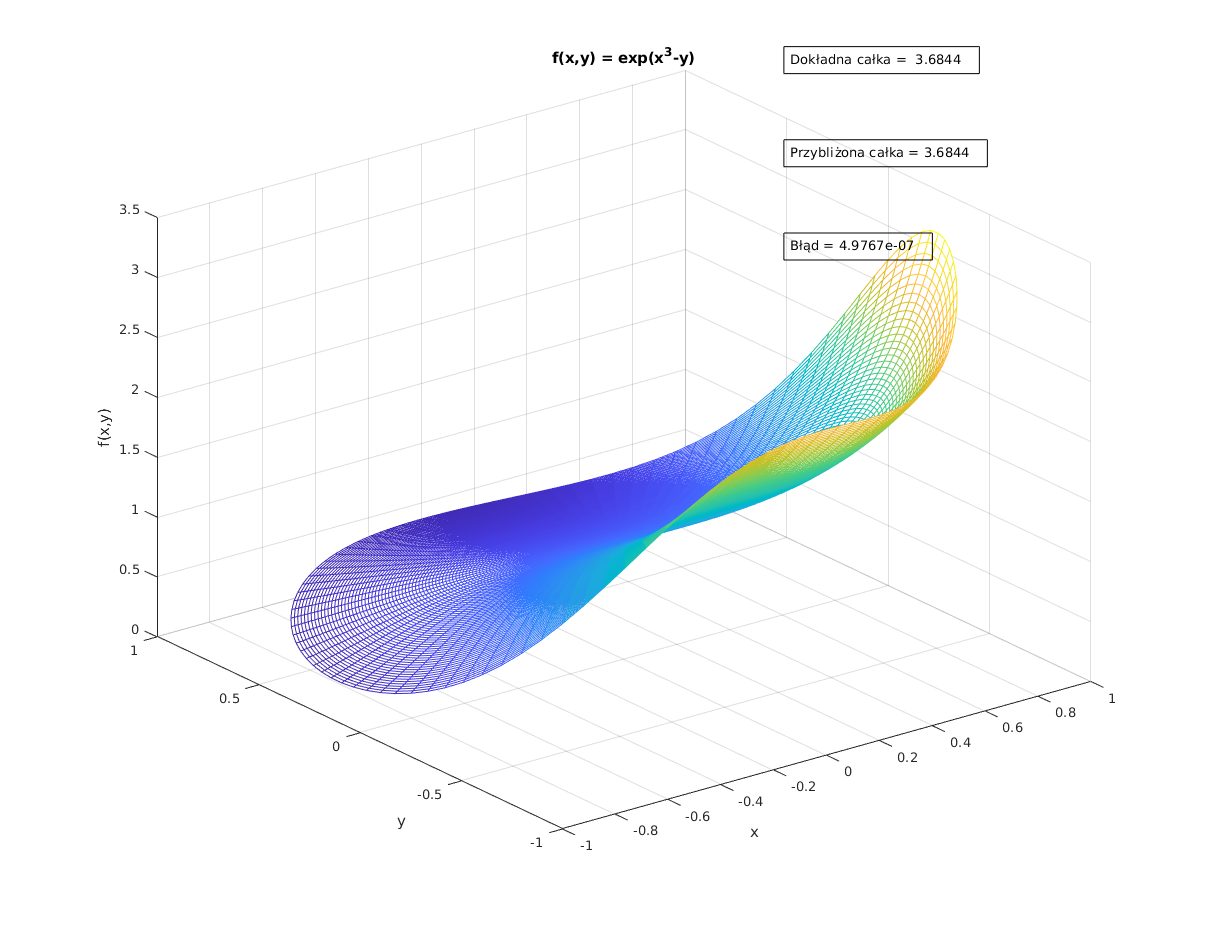
\includegraphics[width = 12cm]{fun1.png}
    \caption{Wynik dla funkcji $f(x,y) = e^{x^3-y}$. Błąd jest bardzo mały, zatem program działa.}
    \label{fun1}
\end{figure}

\begin{figure}[H]
    \centering
    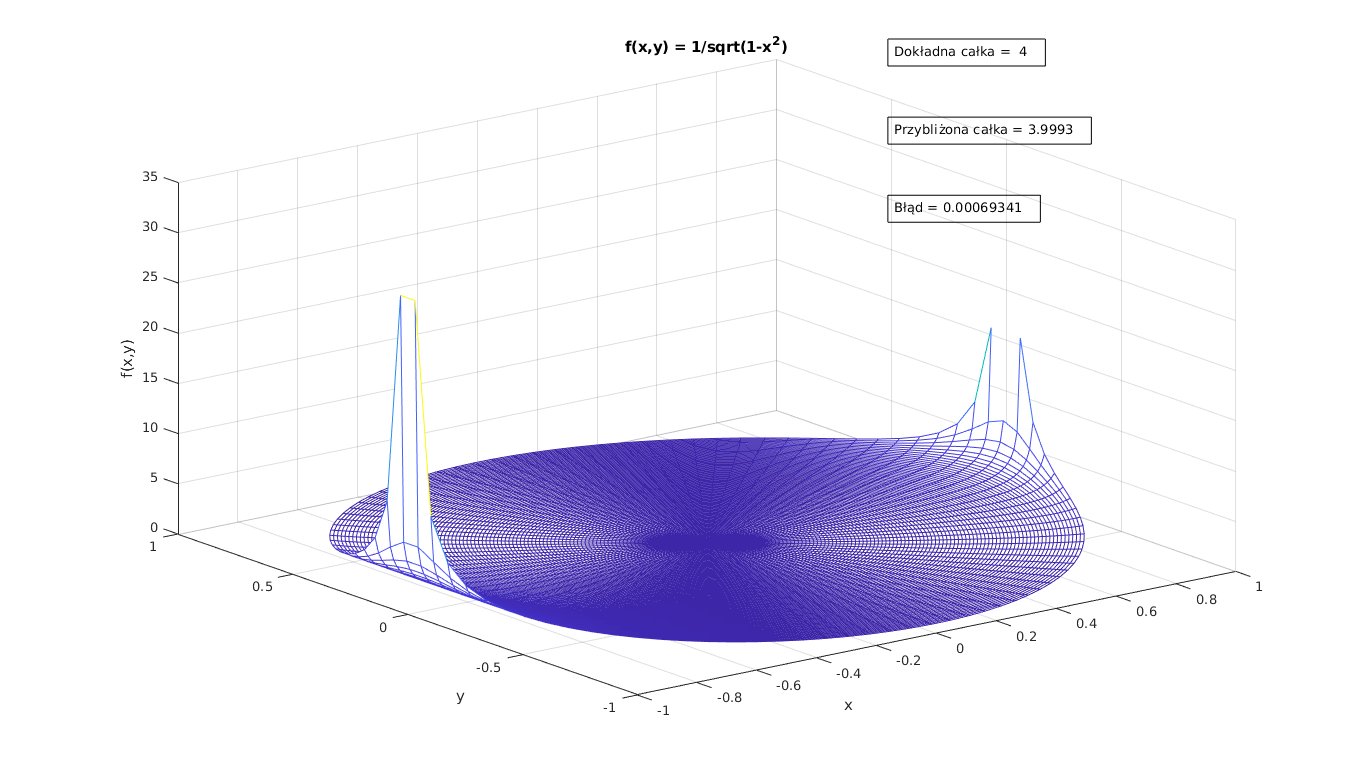
\includegraphics[width = 12cm]{fun2.png}
    \caption{Wynik dla funkcji $f(x,y) = \frac{1}{\sqrt{1-x^2}}$. Błąd jest już trochę większy.}
    \label{fun2}
\end{figure}

\begin{figure}[H]
    \centering
    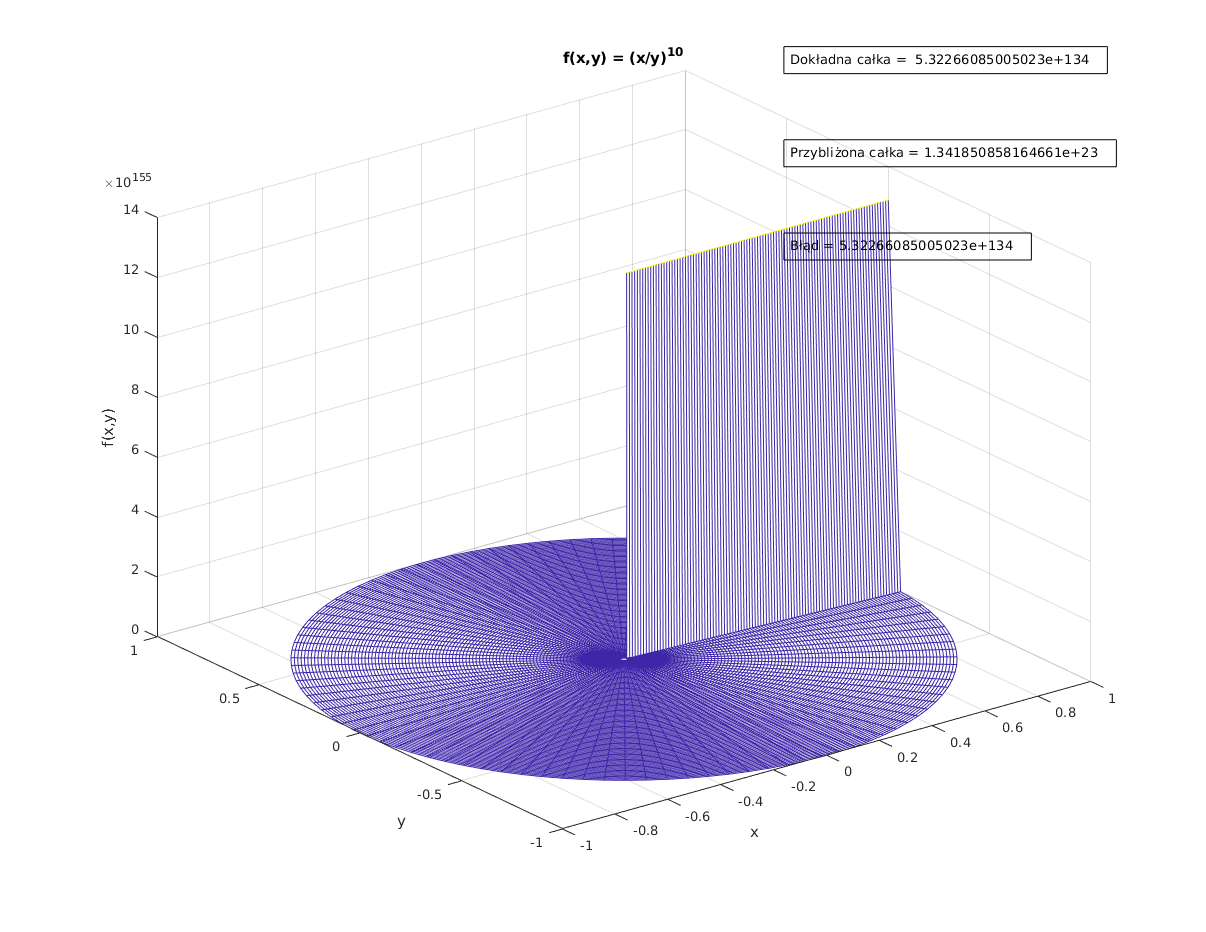
\includegraphics[width = 12cm]{fun3.png}
    \caption{Wynik dla funkcji $f(x,y) = (\frac{x}{y})^{10}$. Program nie radzi sobie z dzieleniem bardzo małych liczb. Błąd jest bardzo duży.}
    \label{fun3}
\end{figure}

\begin{figure}[H]
    \centering
    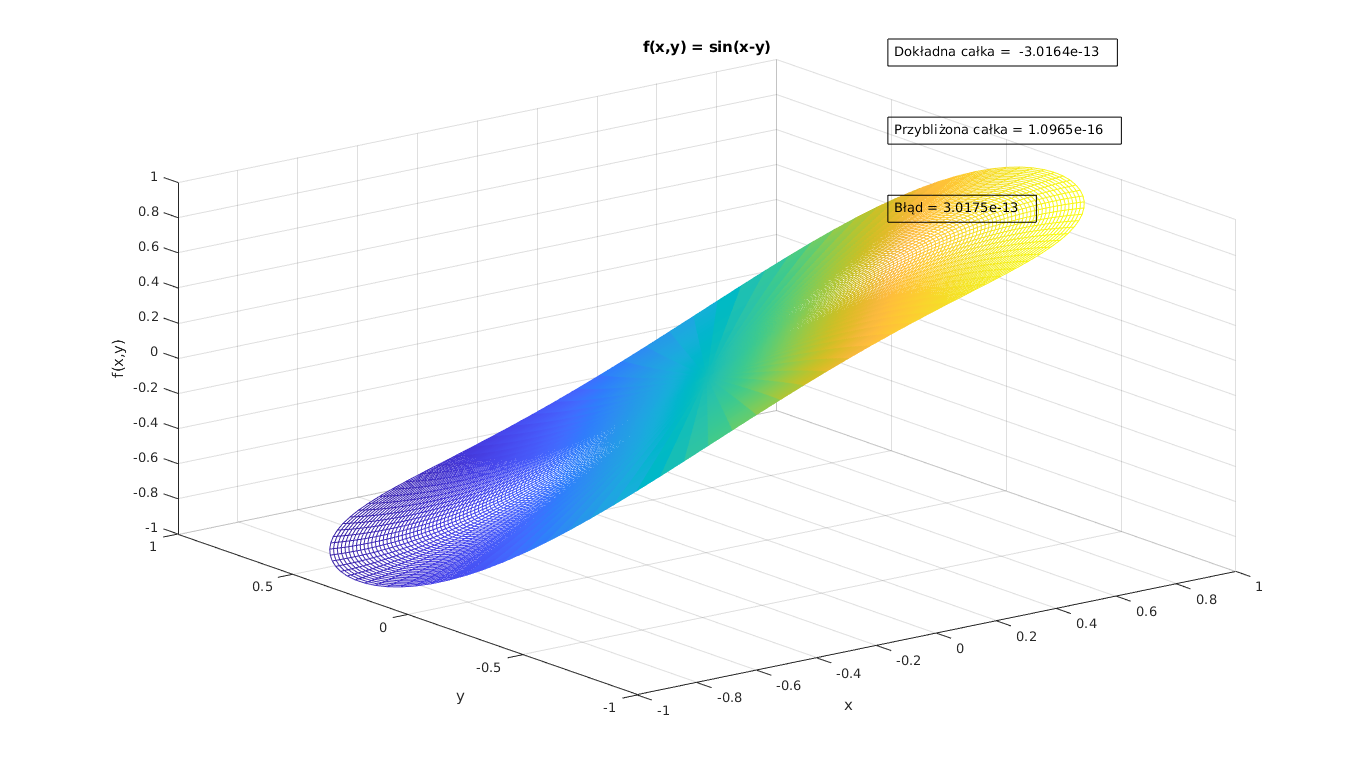
\includegraphics[width = 15cm]{fun4.png}
    \caption{Wynik dla funkcji $f(x,y) = \sin(x-y)$. Program liczy całkę bez problemu. Wartość dokładna i przybliżona różnią się znakiem.}
    \label{fun4}
\end{figure}

\begin{figure}[H]
    \centering
    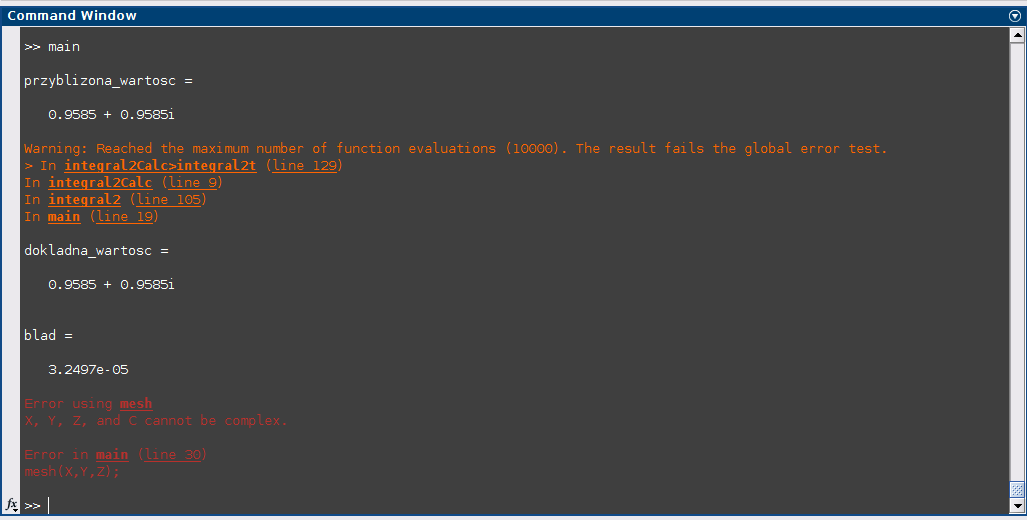
\includegraphics[width = 15cm]{fun5.png}
    \caption{Wynik dla funkcji $f(x,y) = \sqrt{x}+y$. Program daje radę, mimo przejścia na zespolone. Jest już jednak problem z wykresem.}
    \label{fun5}
\end{figure}

\begin{figure}[H]
    \centering
    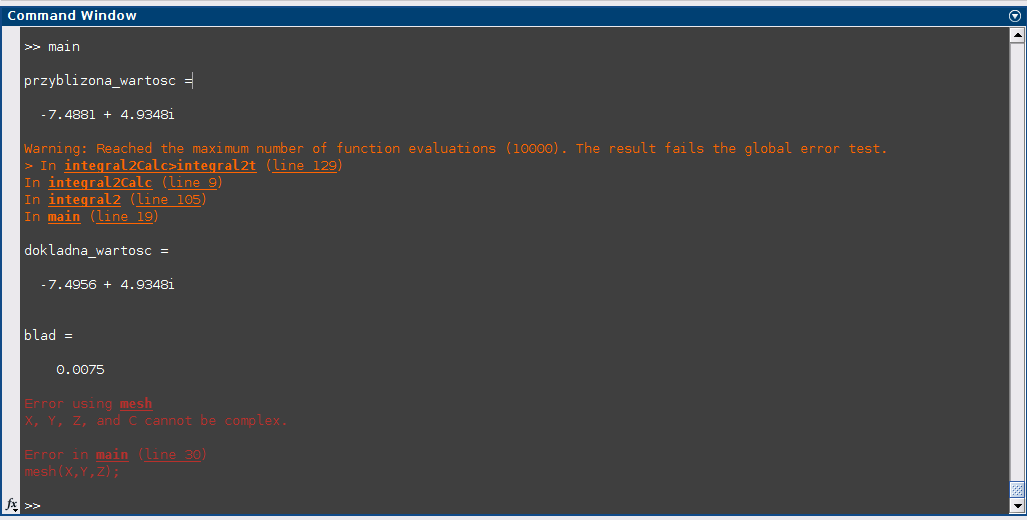
\includegraphics[width = 15cm]{fun6.png}
    \caption{Wynik dla funkcji $f(x,y) = \log(xy)$. Ponownie zespolone. Tutaj już błąd jest znacznie większy.}
    \label{fun6}
\end{figure}

\bigskip



\section{Analiza wynik\'ow}

\begin{table}[h!]
\caption{\footnotesize Wyniki} %\vskip1ex
\renewcommand{\arraystretch}{1.1}
\centering\begin{tabular}{|c|c|c|c|c|}
\hline L.p. & funkcja & wartość & wartość & błąd \\
& & dokładna & przybliżona & \\
\hline 1 & $f(x,y) = e^{x^3-y}$ & 3.6844 & 3.6844 & $4.9767e\!-\!07$ \\
\hline 2 & $f(x,y) = \frac{1}{\sqrt{1-x^2}}$ & 4.0000 & 3.9993 & $6.9341e\!-\!04$ \\
\hline 3 & $f(x,y) = (\frac{x}{y})^{10}$ & $5.3227e\!+\!134$ & $1.3419e\!+\!23$ & $5.3227e\!+\!134$ \\
\hline 4 & $f(x,y) = \sin(x-y)$ & $-3.0164e\!-\!13$ & $1.0965e\!-\!16$ & $3.0175e\!-\!13$ \\
\hline 5 & $f(x,y) = \sqrt{x}+y$ & 0.9585 + 0.9585i & 0.9585 + 0.9585i & $3.2497e\!-\!05
$ \\
\hline 6 & $f(x,y) = \log(xy)$ & -7.4956 + 4.9348i & -7.4881 + 4.9348i & 0.0075 \\
\end{tabular}
\label{Tabela z wynikami algorytmu 1}
\end{table}

W większości przypadków błąd zaimplementowanej kwadratury prostokątów jest mały (rzędu $10^{-4}$ lub mniejszy). Program radzi sobie gorzej z dzieleniem przez bardzo małe liczby (przykład 3). Liczby zespolone nie są jednak aż takim problemem.

\end{document}